\documentclass[a4paper]{article}

\usepackage[english]{babel}
\usepackage[utf8x]{inputenc}
\usepackage{amsmath}
\usepackage{graphicx}
\usepackage[colorinlistoftodos]{todonotes}

\title{Crime Analytics: Visualization of Incident Reports}
%\author{You}

\begin{document}
\maketitle

%\begin{abstract}
%Your abstract.
%\end{abstract}

\section{Introduction}
In this assignment we study the crime incident data set for the city of Seattle in the summer of 2014. Two types of questions are studied and answered. First, we study the temporal patterns of the incidents, i.e. we answered "How do incidents vary by time of day and month to month?" Second, we study the geographical pattern of the crime incidents. Specifically, we answered "How do incidents vary by neighborhood?"
%Your introduction goes here! Some examples of commonly used commands and features are listed below, to help you get started. If you have a question, please use the help menu (``?'') on the top bar to search for help or ask us a question. 

\section{Temporal pattern of Seattle crime incidents}
	\subsection{Daily crime incidents pattern}
%\subsection{How to include Figures}

%First you have to upload the image file from your computer using the upload link the project menu. Then use the includegraphics command to include it in your document. Use the figure environment and the caption command to add a number and a caption to your figure. See the code for Figure \ref{fig:frog} in this section for an example.

It is observed that midnight and noon are two peaks of crime incidents (see Fig.~\ref{fig:dailycrime}). It is also found that 4am - 6am has the fewest incidents. This is probably because criminals need to rest too. By analyzing the data of robbery incidents, we find that robberies are most common around midnight and during 9pm - 11pm. Robberies are least common in the morning around 7am. (see Fig.~\ref{fig:dailyrobbery})

\begin{figure}
\centering
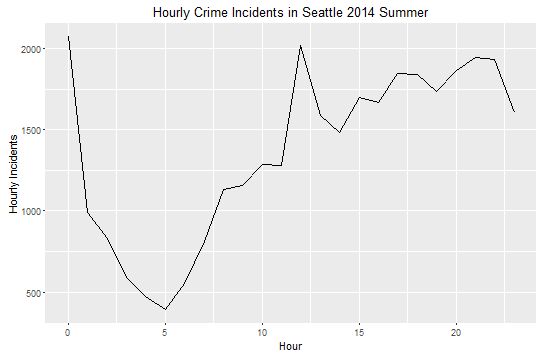
\includegraphics[width=1\textwidth]{HourlyCrime.png}
\caption{\label{fig:dailycrime}Hourly Crime Incidents in the Summer of 2014, Seattle.}
\end{figure}

\begin{figure}
\centering
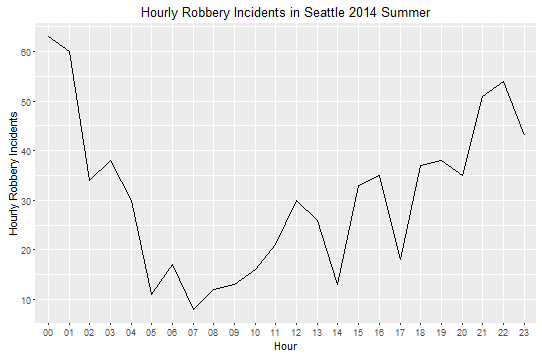
\includegraphics[width=1\textwidth]{HourlyRobbery.png}
\caption{\label{fig:dailyrobbery}Hourly Robbery Incidents in the Summer of 2014, Seattle.}
\end{figure}

	\subsection{Monthly crime incidents}
    In Seattle, the crime incidents did not change much during Summer 2014. As you can see from Fig.~\ref{fig:monthlycrime}, June and July had similar number of crime incidents around 11000, while August had a little smaller number of incidents, about 9000.
 \begin{figure}
\centering
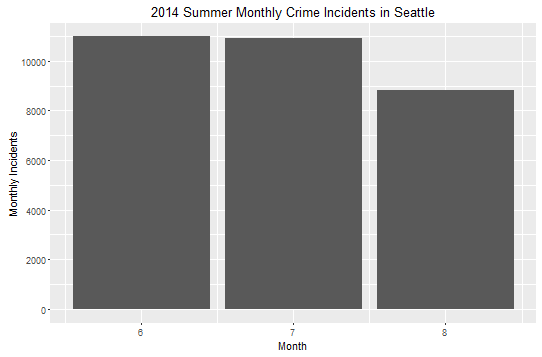
\includegraphics[width=1\textwidth]{MonthlyCrime.png}
\caption{\label{fig:monthlycrime}Monthly Crime Incidents in the Summer of 2014, Seattle.}
\end{figure} 	

\section{Geographical pattern of Seattle crime incidents}
How crime incidents and theft incidents vary by neighborhood is summarized in thermal maps (see Fig. \ref{fig:crimeThermal} and Fig.~\ref{fig:theftThermal}). For general crimes, the top 5 neighborhoods with most incidents are \textbf{Central Business District, Broadway, Belltown, University District} and \textbf{Pioneer Square}. The top 5 neighborhoods with most theft incidents are \textbf{Broadway, University District, Greenwood, Wallingford} and \textbf{Fremont}. Note that Central Business District, Belltown and Pioneer Square belong to the Downtown area and Broadway belongs to the Capitol Hill area. Thus we can conclude that Downtown, Capitol Hill and University District are the top 3 areas with most crime incidents in Seattle. And Capitol Hill and University District are cradle of thefts. 


\begin{figure}
\centering
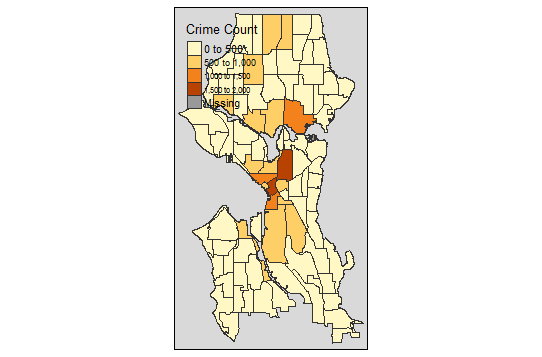
\includegraphics[width=1\textwidth]{crimeMap_s.png}
\caption{\label{fig:crimeThermal}Crime Incidents Thermal Map.}
\end{figure} 

\begin{figure}
\centering
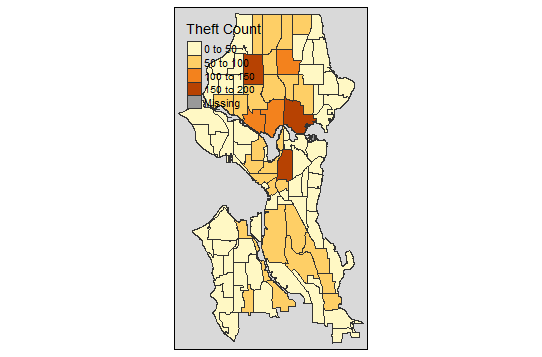
\includegraphics[width=1\textwidth]{theftCount.png}
\caption{\label{fig:theftThermal}Theft Incidents Thermal Map.}
\end{figure} 

%\subsection{How to add Comments}

%Comments can be added to your project by clicking on the comment icon in the toolbar above. % * <john.hammersley@gmail.com> 2016-07-03T09:54:16.211Z:
%
% Here's an example comment!
%
%To reply to a comment, simply click the reply button in the lower right corner of the comment, and you can close them when you're done.

%Comments can also be added to the margins of the compiled PDF using the todo command, \todo{Here's a comment in the margin!} as shown in the example on the right. You can also add inline comments:

%\todo[inline, color=green!40]{This is an inline comment.}

%\subsection{How to add Tables}

%Use the table and tabular commands for basic tables --- see Table~\ref{tab:widgets}, for example. 

%\begin{table}
%\centering
%\begin{tabular}{l|r}
%Item & Quantity \\\hline
%Widgets & 42 \\
%Gadgets & 13
%\end{tabular}
%\caption{\label{tab:widgets}An example table.}
%\end{table}

%\subsection{How to write Mathematics}

%\LaTeX{} is great at typesetting mathematics. Let $X_1, X_2, \ldots, X_n$ be a sequence of independent and identically distributed random variables with $\text{E}[X_i] = \mu$ and $\text{Var}[X_i] = \sigma^2 < \infty$, and let
%\[S_n = \frac{X_1 + X_2 + \cdots + X_n}{n}
%      = \frac{1}{n}\sum_{i}^{n} X_i\]
%denote their mean. Then as $n$ approaches infinity, the random variables $\sqrt{n}(S_n - \mu)$ converge in distribution to a normal $\mathcal{N}(0, \sigma^2)$.


%\subsection{How to create Sections and Subsections}

%Use section and subsections to organize your document. Simply use the section and subsection buttons in the toolbar to create them, and we'll handle all the formatting and numbering automatically.

%\subsection{How to add Lists}

%You can make lists with automatic numbering \dots

%\begin{enumerate}
%\item Like this,
%\item and like this.
%\end{enumerate}
%\dots or bullet points \dots
%\begin{itemize}
%\item Like this,
%\item and like this.
%\end{itemize}

%We hope you find Overleaf useful, and please let us know if you have any feedback using the help menu above.

\end{document}